\section{Распределение баллов}

\subsection{Областной этап. 2022-2023.}
Задания областного этапа можно скачать с \href{https://olympiads.bc-pf.org/chemistry/oblast/2023}{Базы Olympiads}. Во всех графиках баллы представлены в виде \% от максимального. Довольно удивительно, что несмотря на то, что подавляющее большинство участников посчитали задания областного этапа довольно легкими, баллы сконцентрированы в районе нуля и нормальное распределение на наблюдается (несмотря на довольно большую выборку: 432 результата в 9 кл., 347 в 10 кл. и 312 в 11 кл.).

\includegraphics[width=\linewidth]{../export/pdf/results/2023/oblast/grade9-dist-problemwise.pdf}
\newpage

\includegraphics[width=\linewidth]{../export/pdf/results/2023/oblast/grade10-dist-problemwise.pdf}
\includegraphics[width=\linewidth]{../export/pdf/results/2023/oblast/grade11-dist-problemwise.pdf}

\includegraphics[width=\linewidth]{../export/pdf/results/2023/oblast/grade9-dist-box.pdf}
\includegraphics[width=\linewidth]{../export/pdf/results/2023/oblast/grade10-dist-box.pdf}
\includegraphics[width=\linewidth]{../export/pdf/results/2023/oblast/grade11-dist-box.pdf}

Создание этих графиков стало возможным благодаря тому, что РНПЦ Дарын, впервые в истории, начал публиковать протокола областного этапа в общем доступе. К сожалению, у протоколов нет единого формата, некоторые области публиковали только итоговые баллы, половина протоколов была опубликована в PDF формате (из-за чего пришлось потратить десяток часов на перенос результатов в формат таблицы) - но все же это положительный шаг в сторону большей прозрачности олимпиад, и Коллегия выражает благодарность за это. 
\newpage
\subsection{Заключительный этап. 2022-2023.}

\includegraphics[width=\linewidth]{../export/pdf/results/2023/respa/grade9-dist-problemwise.pdf}
\includegraphics[width=\linewidth]{../export/pdf/results/2023/respa/grade10-dist-problemwise.pdf}
\includegraphics[width=\linewidth]{../export/pdf/results/2023/respa/grade11-dist-problemwise.pdf}


\includegraphics[width=\linewidth]{../export/pdf/results/2023/respa/grade9-dist-box.pdf}
\includegraphics[width=\linewidth]{../export/pdf/results/2023/respa/grade10-dist-box.pdf}
\includegraphics[width=\linewidth]{../export/pdf/results/2023/respa/grade11-dist-box.pdf}

\newpage
\subsection{Заключительный этап. 2021-2022.}

Поскольку не мало участников заключительного этапа считает, что заключительный этап в 2022-2023 уч. году был значительно сложнее заключительных этапов в предыдущие годы, мы решили построить аналогичные графики для результатов 2021-2022 и 2020-2021 уч. годов.

\includegraphics[width=\linewidth]{../export/pdf/results/2022/respa/grade9-dist-problemwise.pdf}
\includegraphics[width=\linewidth]{../export/pdf/results/2022/respa/grade10-dist-problemwise.pdf}
\includegraphics[width=\linewidth]{../export/pdf/results/2022/respa/grade11-dist-problemwise.pdf}


\includegraphics[width=\linewidth]{../export/pdf/results/2022/respa/grade9-dist-box.pdf}
\includegraphics[width=\linewidth]{../export/pdf/results/2022/respa/grade10-dist-box.pdf}
\includegraphics[width=\linewidth]{../export/pdf/results/2022/respa/grade11-dist-box.pdf}

\subsection{Заключительный этап. 2020-2021.}

\includegraphics[width=\linewidth]{../export/pdf/results/2021/respa/grade9-dist-problemwise.pdf}
\includegraphics[width=\linewidth]{../export/pdf/results/2021/respa/grade10-dist-problemwise.pdf}
\includegraphics[width=\linewidth]{../export/pdf/results/2021/respa/grade11-dist-problemwise.pdf}


\includegraphics[width=\linewidth]{../export/pdf/results/2021/respa/grade9-dist-box.pdf}
\includegraphics[width=\linewidth]{../export/pdf/results/2021/respa/grade10-dist-box.pdf}
\includegraphics[width=\linewidth]{../export/pdf/results/2021/respa/grade11-dist-box.pdf}

\newpage
\section{Корреляция областного и заключительного этапов}
Нас может интересовать - насколько результаты областного этапа коррелируют с результатами заключительного этапа? Иными словами, насколько хорошо выступление ученика на областном этапе (его баллы), предсказывают баллы этого ученика на заключительном этапе? Оценить корреляцию можно посчитав \href{https://en.wikipedia.org/wiki/Pearson_correlation_coefficient}{коэффициент Пирсона}. Коэффициент Пирсона $\rho$ - нормализованная ковариация двух массивов данных, принимает значение $\rho \in [-1, 1]$. Чем больше $|\rho|$, тем сильнее корреляция. Отрицательные значения $\rho$ показывают обратную корреляцию (например, чем больше баллов на областном этапе, тем меньше баллов на заключительном этапе). Коэффициенты Пирсона для баллов областного и заключительного этапов в 2022-2023 уч. году:

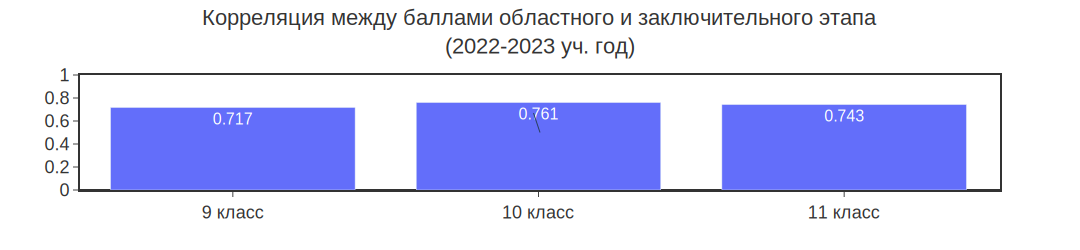
\includegraphics[width=\linewidth]{../export/pdf/trajectory/bygrade.pdf}

Посмотрим как выглядит зависимость графически:

\includegraphics[width=\linewidth]{../export/pdf/trajectory/gr9-data.pdf}
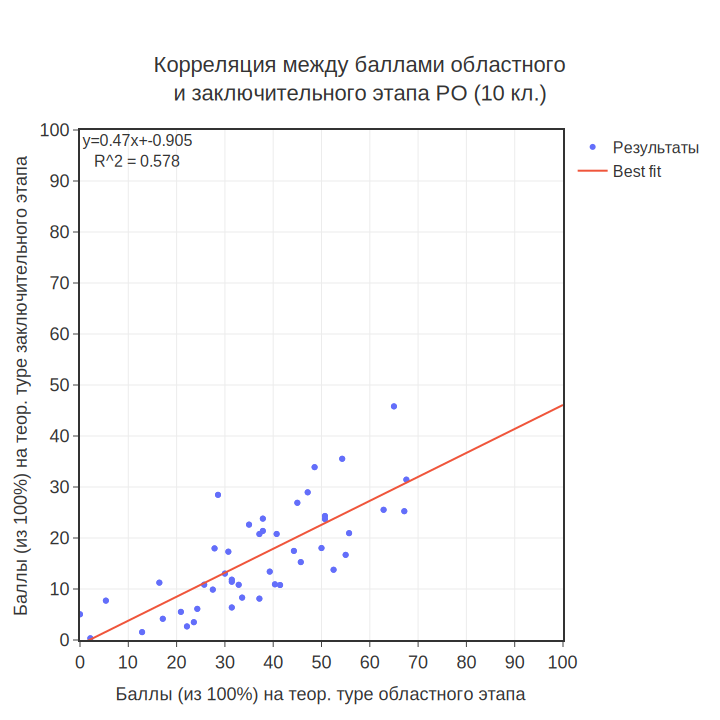
\includegraphics[width=\linewidth]{../export/pdf/trajectory/gr10-data.pdf}
\includegraphics[width=\linewidth]{../export/pdf/trajectory/gr11-data.pdf}

Интересно было бы посмотреть как выглядит эта зависимость в разрезе областей. Поскольку с каждой области и каждого класса на заключительный этап проходит 2-3 человека, считать корреляцию для каждого класса по-отдельности не имеет смысла. Поэтому посчитаем корреляцию для трех классов сразу:

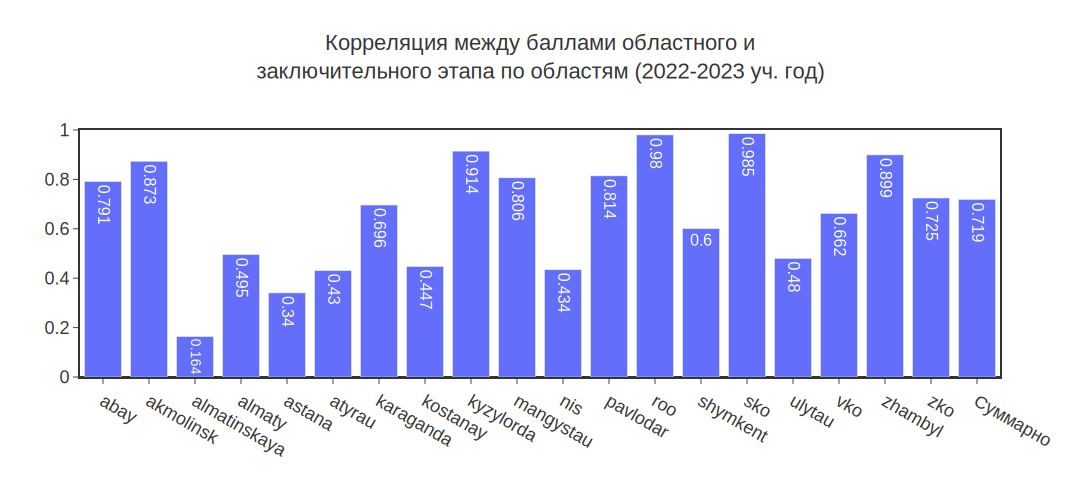
\includegraphics[width=\linewidth]{../export/pdf/trajectory/byoblast.pdf}

Вариация коэффициентов Пирсона поражает. Посмотрим как выглядит зависимость на примере некоторых областей (графики для всех областей есть \href{https://github.com/anmorgunov/respa-data-analysis/tree/main/export/pdf/trajectory}{в публичном репозитории на github}):

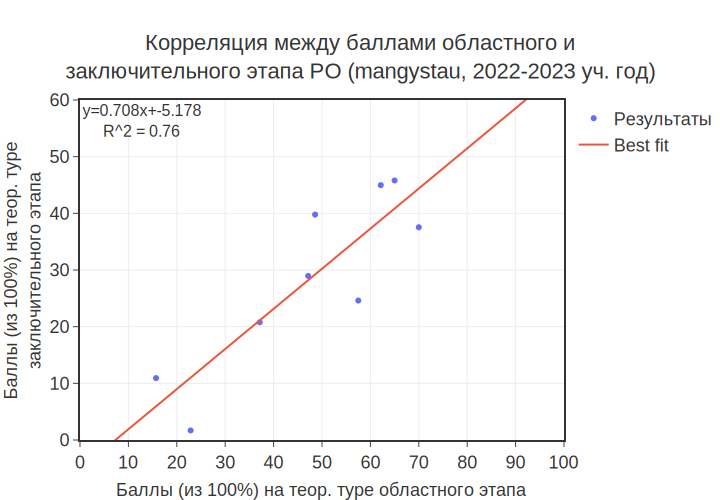
\includegraphics[width=\linewidth]{../export/pdf/trajectory/obl-mangystau.pdf}
\includegraphics[width=\linewidth]{../export/pdf/trajectory/obl-nis.pdf}
\includegraphics[width=\linewidth]{../export/pdf/trajectory/obl-pavlodar.pdf}

\section{Корреляция внутри комплекта заданий}

\subsection{Заключительный этап. 2022-2023.}

А что если посчитать коэффициенты Пирсона внутри одной олимпиады, для баллов за любые две задачи? Большой коэффициент Пирсона (напомним, значения коэффициента находятся в диапазоне от -1 до +1) означает, что если ученик набрал высокий балл по одной задаче, то скорее всего он набрал высокий балл и по другой задаче. С одной стороны, высокую корреляцию можно считать показателем сбалансированности комплекта с точки зрения сложности заданий. С другой стороны, сложно ожидать высокую корреляцию между баллами за задачу, скажем, по неорганической химии и органической химии. 

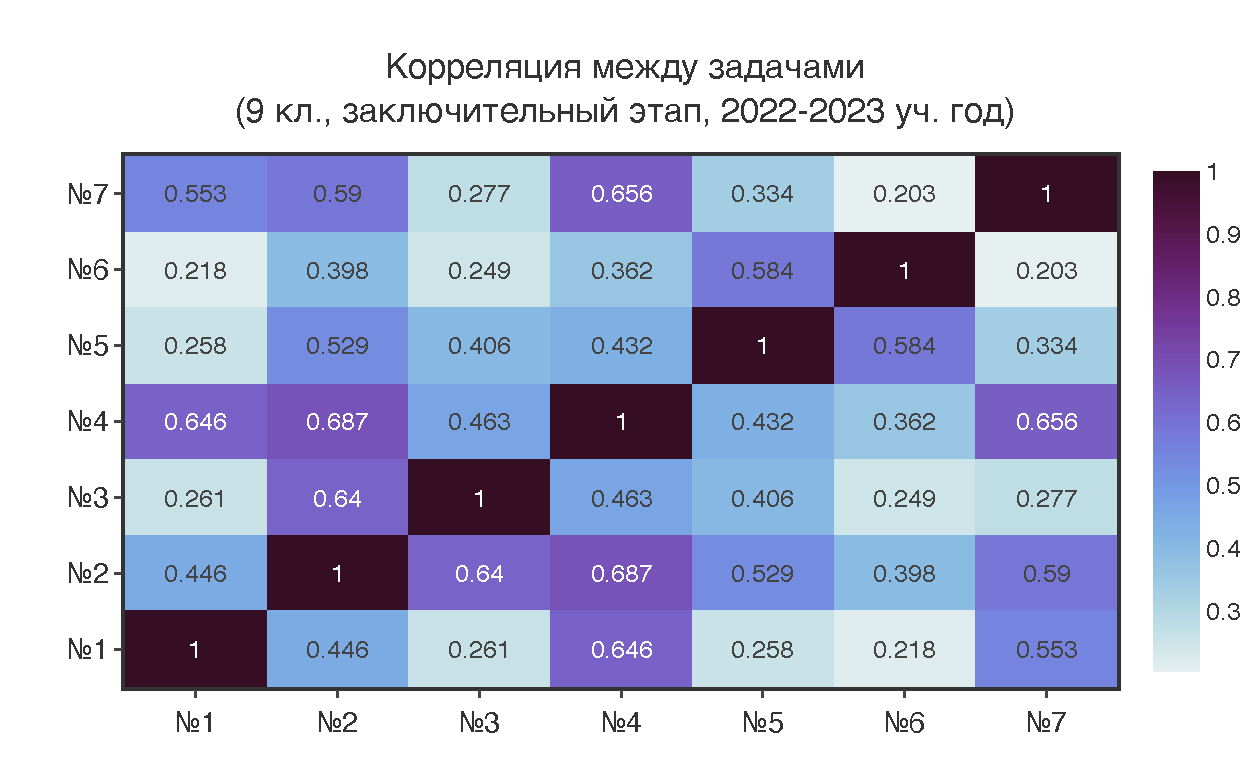
\includegraphics[width=\linewidth]{../export/pdf/results/2023/respa/grade9.pdf}

\newpage

\includegraphics[width=\linewidth]{../export/pdf/results/2023/respa/grade10.pdf}

\includegraphics[width=\linewidth]{../export/pdf/results/2023/respa/grade11.pdf}

\newpage 

А что если мы попробуем посмотреть насколько одна-две любые задачи отличаются от остальных? Возьмем задачу $x$ и задачу $y$, посчитаем средний балл для каждого ученика и сравним со средними баллами за все задачи, кроме задач $x$ и $y$. Полученный коэффициент Пирсона отразим в ячейке $(x,y)$.

\includegraphics[width=\linewidth]{../export/pdf/results/2023/respa/grade9-avg.pdf}

\includegraphics[width=\linewidth]{../export/pdf/results/2023/respa/grade10-avg.pdf}

\includegraphics[width=\linewidth]{../export/pdf/results/2023/respa/grade11-avg.pdf}

\subsection{Областной этап. 2022-2023.}
Повторим те же расчеты для заданий областного этапа.

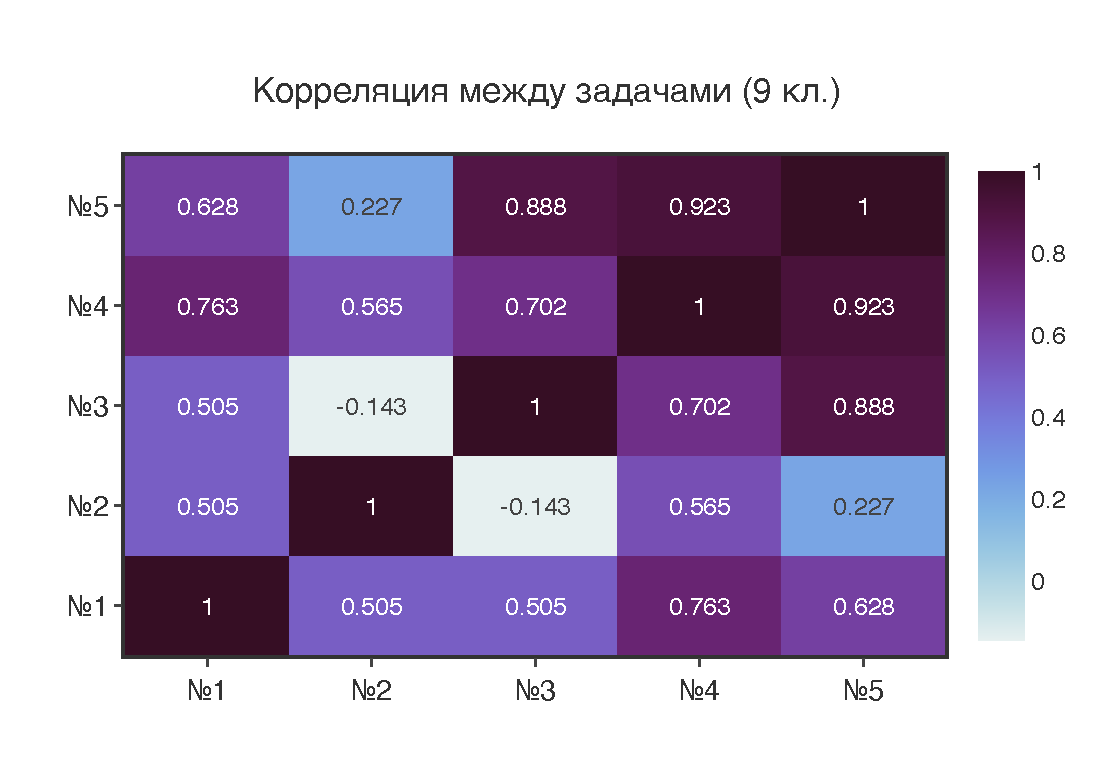
\includegraphics[width=\linewidth]{../export/pdf/results/2023/oblast/grade9.pdf}

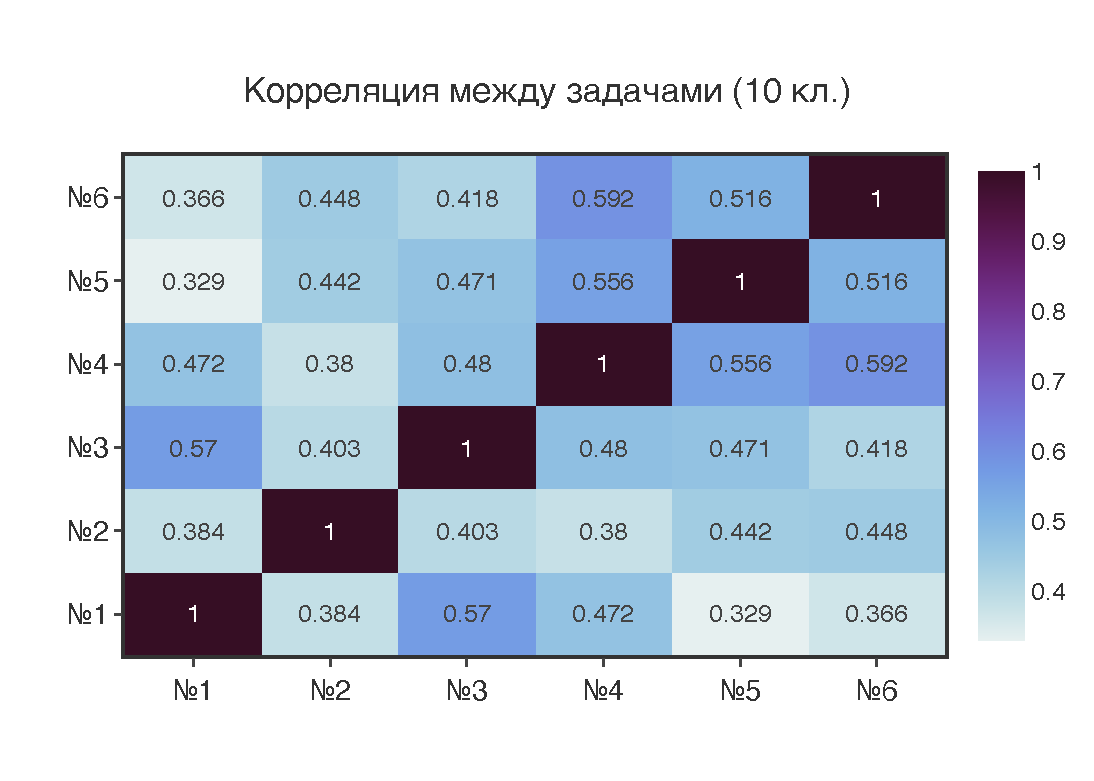
\includegraphics[width=\linewidth]{../export/pdf/results/2023/oblast/grade10.pdf}

\includegraphics[width=\linewidth]{../export/pdf/results/2023/oblast/grade11.pdf}

\includegraphics[width=\linewidth]{../export/pdf/results/2023/oblast/grade9-avg.pdf}

\includegraphics[width=\linewidth]{../export/pdf/results/2023/oblast/grade10-avg.pdf}

\includegraphics[width=\linewidth]{../export/pdf/results/2023/oblast/grade11-avg.pdf}

\subsection{Заключительный этап. 2021-2022.}

Для сравнения, повторим те же расчеты для заключительного этапа 2021-2022 уч. года.

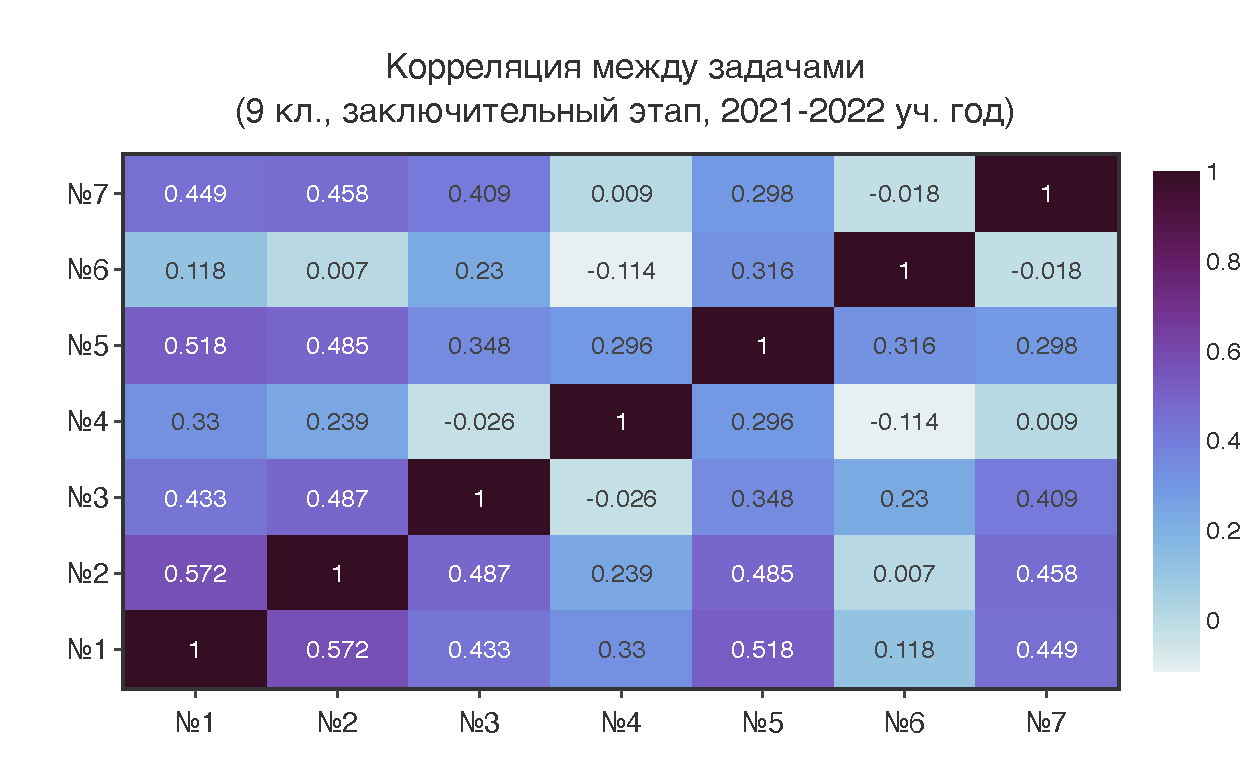
\includegraphics[width=\linewidth]{../export/pdf/results/2022/respa/grade9.pdf}

\includegraphics[width=\linewidth]{../export/pdf/results/2022/respa/grade10.pdf}

\includegraphics[width=\linewidth]{../export/pdf/results/2022/respa/grade11.pdf}

\includegraphics[width=\linewidth]{../export/pdf/results/2022/respa/grade9-avg.pdf}

\includegraphics[width=\linewidth]{../export/pdf/results/2022/respa/grade10-avg.pdf}

\includegraphics[width=\linewidth]{../export/pdf/results/2022/respa/grade11-avg.pdf}

\subsection{Заключительный этап. 2020-2021.}

Для сравнения, повторим те же расчеты для заключительного этапа 2020-2021 уч. года.

\includegraphics[width=\linewidth]{../export/pdf/results/2021/respa/grade9.pdf}

\includegraphics[width=\linewidth]{../export/pdf/results/2021/respa/grade10.pdf}

\includegraphics[width=\linewidth]{../export/pdf/results/2021/respa/grade11.pdf}

\includegraphics[width=\linewidth]{../export/pdf/results/2021/respa/grade9-avg.pdf}

\includegraphics[width=\linewidth]{../export/pdf/results/2021/respa/grade10-avg.pdf}

\includegraphics[width=\linewidth]{../export/pdf/results/2021/respa/grade11-avg.pdf}

\newpage 

\section{Способность учеников к самостоятельной оценке}

В рамках онлайн-опросов, проводившихся в текущем учебном году, ученикам предлагалось оценить насколько хорошо они решили ту или иную задачу выбрав один из четырех вариантов ответов:

\begin{itemize}
    \itemsep-0.3em
    \item[--] Я не решил(а) эту задачу и я даже не знал(а) с чего начать
    \item[--] У меня были идеи по решению задачи, но я не смог(ла) их довести до ума
    \item[--] Я решил(а) задачу, но думаю у меня есть ошибки
    \item[--] Я решил(а) эту задачу и уверен, что решил(а) правильно на 80\% и больше.
\end{itemize}

Нам стало интересно: а насколько эта самооценка коррелирует с истинным результатом? Cначала посмотрим на все классы вместе, а затем на каждый класс по отдельности. Графики для индивидуальных задач есть \href{https://github.com/anmorgunov/respa-data-analysis/tree/main/export/pdf/selfassessment/respa}{в публичном репозитории на github}.

\includegraphics[width=\linewidth]{../export/pdf/selfassessment/respa/allgrade-box.pdf}
\includegraphics[width=\linewidth]{../export/pdf/selfassessment/respa/grade9-box.pdf}
\includegraphics[width=\linewidth]{../export/pdf/selfassessment/respa/grade10-box.pdf}
\includegraphics[width=\linewidth]{../export/pdf/selfassessment/respa/grade11-box.pdf}

Повторим тоже самое для областного этапа:

\includegraphics[width=\linewidth]{../export/pdf/selfassessment/oblast/allgrade-box.pdf}
\includegraphics[width=\linewidth]{../export/pdf/selfassessment/oblast/grade9-box.pdf}
\includegraphics[width=\linewidth]{../export/pdf/selfassessment/oblast/grade10-box.pdf}
\includegraphics[width=\linewidth]{../export/pdf/selfassessment/oblast/grade11-box.pdf}